\documentclass{article}
\usepackage{../fasy-hw}

%% UPDATE these variables:
\renewcommand{\hwnum}{6}
\title{Advanced Algorithms, Homework \hwnum}
\author{Ben Miller}
\collab{\todo{list your collaborators here}}
\date{due: Friday, 19 November 2021}

\begin{document}

\maketitle

This homework assignment should be
submitted as a single PDF file both to D2L and to Gradescope.

General homework expectations:
\begin{itemize}
    \item Homework should be typeset using LaTex.
    \item Answers should be in complete sentences and proofread.
    \item You will not plagiarize, nor will you share your written solutions
        with classmates.
    \item List collaborators at the start of each question using the
        \texttt{collab} command.
    \item Put your answers where the \texttt{todo} command currently is (and
        remove the \texttt{todo}, but not the word \texttt{Answer}).
    \item If you are asked to come up with an algorithm, you are
        expected to give an algorithm that beats the brute force (and, if possible, of
        optimal time complexity). With your algorithm, please provide the following:
        \begin{itemize}
            \item \emph{What}: A prose explanation of the problem and the algorithm,
                including a description of the input/output.
            \item \emph{How}: Describe how the algorithm works, including giving
                psuedocode for it.  Be sure to reference the pseudocode
                from within the prose explanation.
            \item \emph{How Fast}: Runtime, along with justification.  (Or, in the
                extreme, a proof of termination).
            \item \emph{Why}: Statement of the loop invariant for each loop, or
                recursion invariant for each recursive function.
        \end{itemize}
    \item The lowest HW grade is dropped.  However, this HW can only be dropped
        if the grade is at least 25\%.  (In other words, please do not choose to
        drop this homework by not doing any of it).
    \item This homework is an \textbf{individual} assignment.
\end{itemize}

\collab{TODO}
\nextprob{Describe an Algorithm}

Choose one concept or algorithm that you have learned
in this class so far. A student who has
taken 232 and 246, but not 432, has some questions about this problem:

\begin{enumerate}
    \item \emph{What} is the problem that this algorithm solves?

        \paragraph{Answer}
        I'm going to describe the concept of backtracking. Before this class, I did
        not have a very good grasp on this concept and how it differs from recursion.

        Backtracking builds on recursion by taking a problem and slowly exploring
        all the possible paths to reach the best answer.

        Backtracking is solving a problem through exploration with constraints rather than pure
        computation.

    \item \emph{How} does it work? (Describe in prose, with or without
        psuedocode.)

        \paragraph{Answer}
        To illustrate how backtracking works, I'm going to use the N Queens problem
        from the textbook.

        A naive recursive algorithm might try every possible combination of queen
        positions in a recursive loop and evaluate them to see if there are colisions. This would be
        extremely slow and wouldn't take advantage of the constraints of the problem.

        To use backtracking, we initially only put one queen on the board. Then,
        we cross out all the squares that this queen blocks and recurse. This lets
        us not waste time on already blocked squares.

        Another example where backtracking saves the day is in maze solving. We
        can use backtracking to fully explore paths and mark them as explored along
        the way. This way, when we unwind the recursive stack, we can skip exploring
        already explored areas.

        At the end of the day, backtracking is just using the constraints of the
        problem to avoid calculating the same thing twice.

\end{enumerate}


\collab{Weights on Vertices}
\nextprob{}

Chapter 8, Question 3, Part (a).

3. Suppose we are given an undirected graph G in which every vertex has a
positive weight.

(a) Describe and analyze an algorithm to find a spanning tree of G with
minimum total weight. (The total weight of a spanning tree is the sum
of the weights of its vertices.)

\paragraph{Answer}

For this algorithm, we will start with an arbitrary vertex and repeatedly add
the smallest edge to our tree. This is pretty much Jarnik's algorithm. All
of the minimum spanning tree algorithms esentially revolve around adding safe edges
in the graph. By progressing through the graph with just our tree starting at our
initial vertex, a safe edge will always be the smallest edge from the tree to another
unvisited vertex.

\begin{algorithm} \caption{\textsc{Jarnik's/Ben's minimum spanning tree} (G (E, V, w))}\label{alg:seb}
    {\bf Input:} A weighted undirected graph with positive weights\\
    {\bf Output:} A minimum spanning tree.
    \begin{algorithmic}[1]
        \State$select\ start\ vertex\ and\ initialize\ subgraph\ T$
        \State$Initialize\ priority\ queue$
        \For{$i \gets 1\ to\ |V| -1$}
            \State$v \gets PriorityQueueMin$
            \If{$v \notin T$}
                \State$add\ v\ and\ edge_v\ to\ T$
                \State$add\ edges\ not\ to\ T\ to\ PriorityQueue$
            \EndIf{}
        \EndFor{}
    \end{algorithmic}
\end{algorithm}

We interact with every vertex and every edge, so we immediately have O(V+E). By
marking the vertices when we add them to T, we can determine if a vertex is in T
i O(1) time. Extracting and adding to the priority queue can be done in O(logv) time
which is done on each vertex, so the overall running time is O(E+VlogV)

\nextprob{MED}
Consider the randomized minimum enclosing disc (MED) algorithm.  In this
homework, we investigate the worst-case analysis of it.  In class, we will study
the randomized analysis.

\begin{algorithm}\caption{\textsc{MED($S$, $\Sigma$)}}\label{alg:seb}
    {\bf Input:} two finite sets $S$, $\Sigma \subset \R^2$\\
    {\bf Output:} $B$, the smallest ball enclosing $S$ with points of
    $\Sigma$ on the boundary.

    \begin{algorithmic}[1]
        \If{$|S|=0$}\\
        ~~~~~~\Return the smallest ball with $\Sigma$ on boundary
        \EndIf

        \State $i \gets \textsc{Random}(n)$
        \State $B = \textsc{MED}(S \backslash S[i], \Sigma)$
        \If{$S[i] \in B$}\\
        ~~~~~~\Return $B$
        \Else\\
        ~~~~~~\Return $\textsc{MED}\left((S \backslash S[i], \Sigma \cup \{ S[i]
        \}\right)$
        \EndIf
    \end{algorithmic}
\end{algorithm}

In the above algorithm, suppose $\textsc{Random}(n)$ returns a random integer
between $1$ and $n$ (inclusive).  Further suppose
$S$ is stored as an array with indices $1$ though $n$,
and $|\Sigma| \leq 3$.  Let's represent the output ball as an ordered
pair~$B=(b_c,b_r) \in \R^2 \times \R_{\geq 0}$,
where $b_c\in \R^2$ is the center of a smallest enclosing ball and $b_r$ is the
radius of the smallest enclosing ball.

\begin{enumerate}[(a)]
    \item
        Suppose $S=\emptyset$ and $\Sigma=\{ (a_x,a_y)\}$. What ball is returned on Line 2?
        \paragraph{Answer} The ball is centered on $(a_x,a_y)$ with radius zero. $B = ((a_x,a_y), 0)$
    \item
        Suppose $S=\emptyset$ and $\Sigma=\{ a=(a_x,a_y),b=(b_x,b_y)\}$, what ball is returned on Line 2?
        \paragraph{Answer}
        The ball whose center is between a and b with a radius of the distance to a.\\
        $B = (j = (\frac{a_x + b_x}{2},\frac{a_x + b_x}{2}), dist(j, x))$
    \item
        Suppose $S=\emptyset$ and $\Sigma=\{ a=(a_x,a_y),b=(b_x,b_y)\}$, what ball is returned on Line 2?
        \paragraph{Answer}
        Same as last question?\\
        The ball whose center is between a and b with a radius of the distance to a.\\
        $B = (j = (\frac{a_x + b_x}{2},\frac{a_x + b_x}{2}), dist(j, x))$
    \item Let $T(n)$ be the time complexity of MED($S$, $\Sigma$) when
        $|S|=n$.  Give the worst-case recurrence~relation.\label{recursive-form}
        \paragraph{Answer} $MED(n) = 2 \cdot MED(n-1) + \Theta(1)$\\
        The worst case would be if S[i] $\notin$ B for each recursive loop, which means every point is on the boundary.
    \item What is the asymptotic form of your answer to (\ref{recursive-form})?
        \paragraph{Answer} $O(2^n)$
\end{enumerate}


\collab{TODO}
\nextprob{Algorithms in the News}

Find an algorithm discussed in a recent news article (over the past 12 months).
Choose ONE of the following:
\begin{enumerate}
    \item Look up the primary resource for this algorithm (likely to be a
        research paper).  Compare/contrast the similarities and differences between the
        way the news article describes the problem and algorithm with the way
        that the primary resource describes it.
    \item If the algorithm itself is not given in the article, provide a prose
        description of the algorithm along with pseudocode. (This might require
        looking up the primary resource for the algorithm).
    \item Analyze the runtime of the algorithm.
    \item Prove the correctness of the algorithm.
\end{enumerate}

\paragraph{Answer}
\todo{answer here}

\collab{TODO}
\nextprob{Decrementing Function}

Prove that the generic algorithm for SSSP, \textsc{FordSSSP}, terminates using a
decrementing function.

\paragraph{Answer}

\begin{algorithm} \caption{\textsc{FordSSSP} (s)}\label{alg:seb}
    {\bf Input:} source vertex\\
    {\bf Output:} distances to vertices
    \begin{algorithmic}[1]
        \State$InitSSSP(s)$
        \While{$there\ is\ at\ least\ one\ tense\ edge$}
            \State$relax\ any\ tense\ edge$
        \EndWhile\\
    \end{algorithmic}
\end{algorithm}

"an edge u to v is tense if dist(u)+w(u to v) $<$ dist(v)."

$$d : \mathcal{S} \rightarrow \mathbb{R}$$
$$d(\matchcal{S_{i+1}}) < d(\matchcal{S_i})$$

For every loop through FordSSSP, the sum of the distances to each vertex decreases.
Each pass relaxes a tense edge which reduces the total distance of the graph. Once
the total distance is at its minimum, there will be no more tense edges to relax
and the algorithm will terminate.

\collab{TODO}
\nextprob{All Pairs Shortest Paths}

Walk through \textsc{ShimbelAPSP} algorithm (Erickson, page 314) for the graph given in class on
11/10/21.

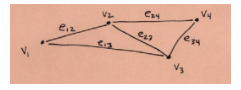
\includegraphics[width=250,height=400,keepaspectratio]{432-111021-graph.png}

\paragraph{Answer}

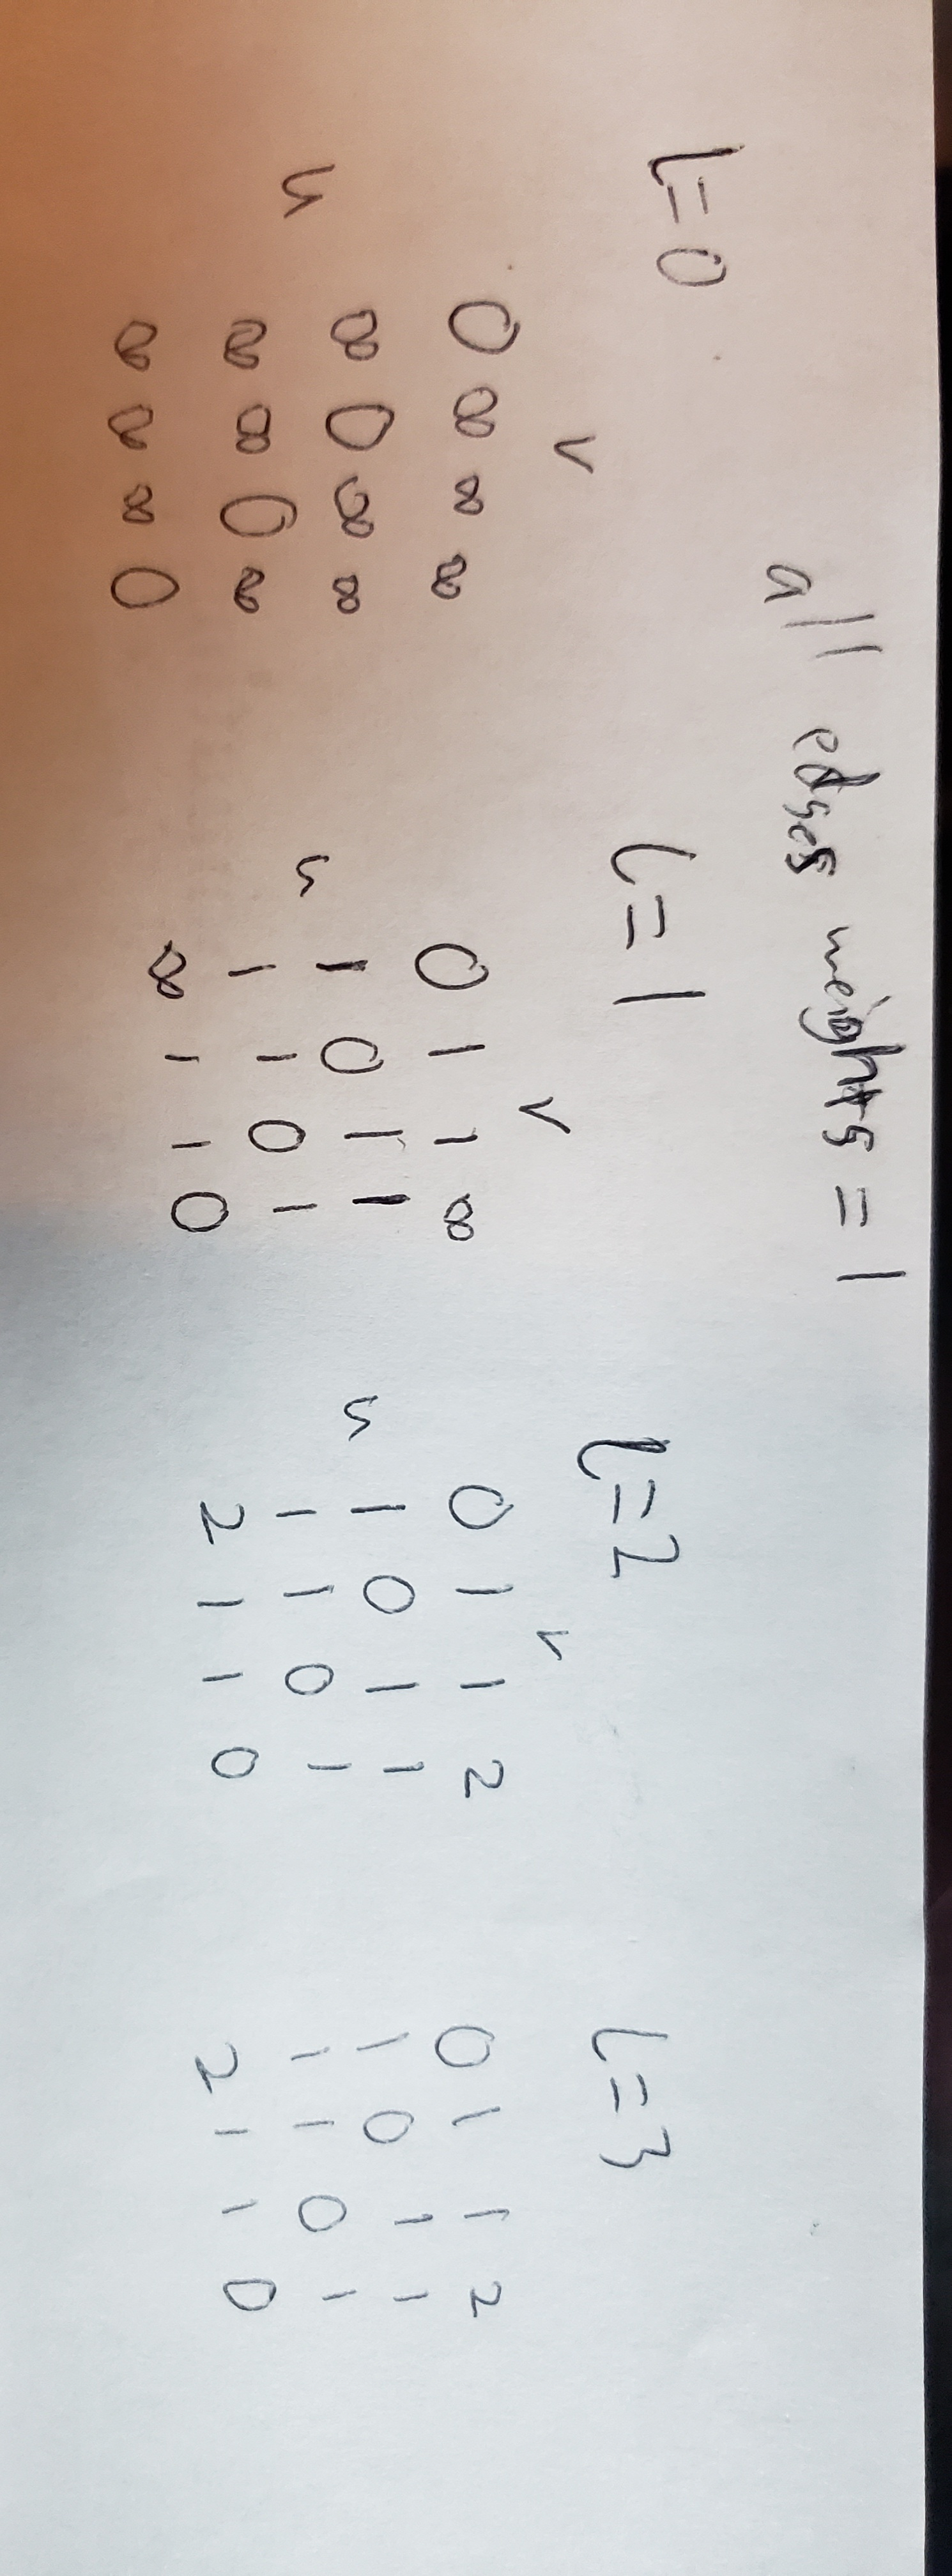
\includegraphics[width=250,height=400,keepaspectratio,angle=90]{q6Walkthrough.jpg}
\end{document}
